\chapter{Realizace}
\label{realizace}
% promereni zapojeni jestli vse funguje 
% TODO + struktura firmware a provadeni digitalniho testu -> KAM TO ZARADIT? mozna do subsection realizace?
V této části bude popsána detailní realizace celého zařízení. V předchozích částech byly zmíněny základní požadavky na návrh celého vyčítacího rozhraní. Při výběru individuálních částí rozhraní byly tyto části respektovány. Dále jednotlivé části byly vybírány s ohledem na miniaturizaci rozhraní a spotřebu. Cílem návrhu bylo pokud co možno nejvíce funkčních bloků implementovat na základní desce. Prvním důvodem bylo, že druhá deska plošných spojů (chipboard) obsahuje detektor Timepix 2, který je v celém návrhu nejdůležitější a nejsložitější částí. Pokud by bylo vše implementováno na jedné desce plošných spojů, při jakémkoliv problému musí být vyměněna celá deska i s detektorem Timepix 2. Přitom při rozložení rozhraní na dvě desky plošných spojů dojde při případném problému k výměně jen základní desky. 
\par Druhým důvodem rozložení rozhraní na dvě desky plošných spojů je minimalizace rozměrů rozhraní. Za použití konektoru celé rozhraní zvýší své rozměry pouze na výšku o 3 mm přitom rozměry chipboardové desky mohou být stejné jako desky základní.

\section{Základní deska}	
	Základní deska je navržena na šesti vrstvém plošném spoji. Využití jednotlivých vrstev lze vidět na obrázku \ref{tab:pcb_vrstvy}. Celková tloušťka výsledného PCB je dle celkové skladby z obrázku \ref{fig:PCB_mother_stackup}, 1.6 mm. Vnější rozměry základní desky jsou 53 x 17 mm.

\begin{figure}
	\begin{minipage}[b]{.45\linewidth}
		\centering
		\captionsetup{justification=centering}
		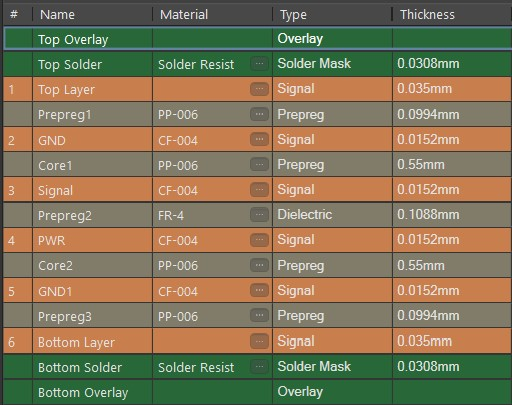
\includegraphics[scale=0.60]{PCB_mother_stackup.jpg}
		\caption{Rozložení vrstev PCB základní desky} 
		\label{fig:PCB_mother_stackup}
	\end{minipage}\hfill
	\begin{minipage}[b]{.45\linewidth}
		\centering
		\begin{tabular}{ |P{3cm}||P{3,5cm}|  }
			\hline
			\multicolumn{2}{|c|}{Rozložení vrstev PCB základní desky} \\
			\hline
			Vrstva  & Popis\\ \hline \hline 
			1 - TOP& Signálová vrstva\\ \hline		
			2 - GND1& Zemní vrstva \\ \hline 		 
			3 - SIG& Signálová vrsta \\ \hline
			4 - PWR& Napájecí vrstva\\ \hline
			5 - GND2& Zemní vrstva\\ \hline
			6 - BOT& Signálová vrstva\\ \hline
		\end{tabular}
		\caption{Popis vrstev PCB základní desky}
		\label{tab:pcb_vrstvy}
	\end{minipage}
\end{figure}

	\subsection{Napájení}
	Na základní desce je realizováno veškeré napájení, které je dále používáno pro celé výčítací rozhraní. Celkem jsou zde tři spínané synchronní buck regulátory. Konkrétně se jedná o regulátor MP2333H \cite{MPH2333} od společnosti Monolithic Power Systems. Regulátor pracuje v rozsahu vstupních napětí on 4.2 - 18 V. maximální výstupní proud jsou 3 A, spínací frekvence regulátoru je 1.2 MHz. Regulátor je možné pořídit v pouzdře SOT583, s rozměry 1.6x2 mm, které jsou pro úlohu minimalizace zařízení vyhovující. V tabulce \ref{tab:napajeni} můžete vidět seznam napětí dostupných na základní desce.
	\begin{table}[h!]
		\centering
		\begin{tabular}{ |P{3cm}||P{10cm}|  }
			\hline
			\multicolumn{2}{|c|}{Napájení základní desky vyčítacího rozhraní} \\
			\hline
			Napájení  & Popis\\ \hline \hline 
			+5V & Externí napájení vyčítacího rozhraní přes USB typu C. \\ \hline		
			+3V3 & Napájení pro mikrokontrolér, CPLD a další 3.3V periférie \\ \hline 		 
			+2V5 & Napájení vstupní a výstupní brány detektoru Timepix 2 \\ \hline
			+1V2 & Napájení jádra Timepix 2 a vstupní/výstupní brány CPLD.\\ \hline
		\end{tabular}
		\caption{Napájení základní desky vyčítacího rozhraní}
		\label{tab:napajeni}
	\end{table}
	Všechny napájení uvedené v tabulce \ref{tab:napajeni} jsou dostupné také na druhé desce, chipboardu. Více o propojení základní desky a chipboardové desky v části \ref{konektor}. Ukázkové zapojení jednoho ze tří spínaných regulátorů, můžete vidět na obrázku \ref{fig:mp2333h}. Konkrétně se jedná o zapojení, při kterém regulátor reguluje +5 V napájení na napájení +1.2 V.
	\begin{figure}[h!]
		\centering
		\captionsetup{justification=centering}
		\includegraphics[scale=0.80]{mp2333h.jpg}
		\caption{Zapojení regulátoru MP2333H} 
		\label{fig:mp2333h}
	\end{figure}
	\subsubsection{Napájecí sekvence}
	Napájecí sekvenci je možné vidět na zjednodušeném diagramu na obrázku \ref{fig:napajeci_sekvence}. Po připojení USB typu C do konektoru na základní dece je dostupné napájení +5 V. Těchto +5 V spíná první regulátor, který generuje na výstupu +3.3 V napájení. Pokud je toto výstupní napájení +3.3 V v pořádku, integrovaný obvod tuto informaci signalizuje pomocí pinu PG. Právě tento pin PG, signál PG\_3V3, je připojen na vstupní pin dalšího regulátoru v sérii a to na pin regulátoru generující výstupní napětí +2.5 V. Poslední regulátor s výstupním napětí +1.2 V je řízený z mikrokontroléru, jeho vstupní pin EN je propojen signálem EN\_1V2 s výstupní bránou mikrokontroléru.
	\begin{figure}[h!]
		\centering
		\captionsetup{justification=centering}
		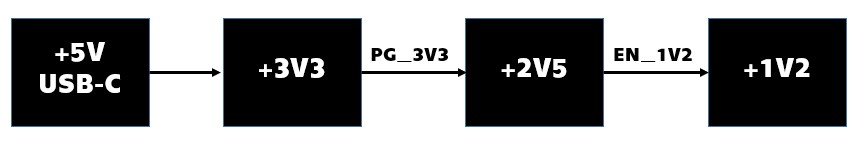
\includegraphics[scale=0.80]{napajeci_sekvence.jpg}
		\caption{Napájecí sekvence základní desky} 
		\label{fig:napajeci_sekvecne}
	\end{figure}
	\par Výstupní napětí spínaného regulátoru je nastaveno pomocí napěťového děliče ve zpětné vazbě regulátoru a dáno vztahem dle \ref{eq:Vout}. Kde $V_{REF}$ = 805 mV.
	\begin{equation}
		V_{OUT} = \frac{R1 \cdot V_{REF}}{R2} + V_{REF}
		\label{eq:Vout}
	\end{equation}

	\par Z obrázku \ref{fig:napajeci_sekvecne} je vidět, že spínaná stabilizátory pro +3.3 V a +2.5 V nejsou programově ovladatelné z mikrokontroléru. Spínaný stabilizátor +3.3 V, z mikrokontroléru řídit nelze, protože právě těchto +3.3 V je napájením pro vybraný mikrokontrolér. Možností jakým mimo jiné zajistit dodržení vhodného časování napájecí sekvence základní desky, je propojení PG signálu stabilizátoru +3.3 V na signál EN stabilizátoru +2.5 V. Další možností rozfázování napájecí sekvence je volba vhodného kondenzátoru mezi pinem SS a zemním pinem ze zapojení \ref{fig:mp2333h}. Kde $V_{REF}$ = 805 mV a $I_{SS}$ = 7.3 $\mu$A.
	\begin{equation}
		T_{SS}\,[ms] = \frac{2V_{REF} \cdot C_{SS} \,[nF]}{I_{SS}}
		\label{eq:Tss}
	\end{equation}
	Ze zapojení \ref{fig:mp2333h} a dosazení do vzorce \ref{eq:Tss} můžeme dopočítat, že rozběhový čas spínaného zdroje bude 1.4 ms. % TODO promerit Tss!!!
	
	\par Ochrana vstupního napájení bude popsána v části \ref{USB}. Pouze ve shrnutí, pokud dojde k jakýmkoliv podmínkám které by mohli elektricky ohrozit vyčítací rozhraní obvody z části \ref{USB} zajistí vypnutí napájení pomocí externího tranzistoru.
	
	%TODO spabilita napapájení

	\subsection{Mikrokontrolér}
	Mikrokontrolér pro tuto práci byl vybrán od firmy STMicroelectronics, přesněji mikrokontrolér s označením STM32U5A9NJH6Q \cite{STM32U5A9}. Právě tento mikrokontrolér byl vybrán s ohledem na požadavky vyčítacího rozhraní. V následující části budou uvedeny nejdůležitější parametry vybraného mikrokontroléru:
	%\vspace{-5mm}
	\begin{itemize}
		\setlength\itemsep{0.005em}
		\item Jádro : Arm 32-bit Cortex-M33 s DSP a FPU. Frekvence 160 MHz
		\item Napájení 1.7 - 3.6 V
		\item Při provozu 18.5 $\mu$A/MHz
		\item 4-Mbyte flash s EEC
		\item 2514-Kbyte RAM, 66 Kbytes s EEC
		\item 25 Komunikačních periférií
		\item 156 konfigurovatelných vstupních/výstupních pinů
		\item 1 USB OTG high-speed s embedded PHY 
		\item Pouzdro : TFBGA216. 13 x 13 mm, 0.8 mm mezi pájecími plošky
	\end{itemize}
	\par Prvním požadavkem na mikrokontrolér bylo, aby bylo možné komunikovat přes sériovou datovou linku s detektorem Timepix 2. V již popsané části textu \ref{Komunikacni rozhrani}, bylo zmíněno, že Timepix 2, dokáže komunikovat po sériové lince s maximální frekvencí 100 Mhz. Výše popsaný vybraný mikrokontrolér umožňuje konfiguraci komunikačního kanálu, konkrétně specfikace SPI až do frekvence 160 MHz. 
	\par Dalším důležitým parametrem při výběru mikrokontroléru byla velikost paměti. Pro vyčtení jedné matice pixelů z detektoru Timepix 2, z výše popsané části textu \ref{Digitálni cast} vyplývá, že je zapotřebí vyčíst 28x256x256 bitů dat, tedy 229.376 kB. Výše vybrané parametry pamětí mikrokontroléru jsou pro tento objem dat dostačující.
	\par Nejméně důležitým parametrem při výběru mikrokontroléru byl parametr integrovaného USB přímo uvnitř mikrokontroléru. Není tedy zapotřebí při návrhu USB umísťovat další součástky, až na ESD ochranu, pro implementaci USB komunikace. Tímto parametrem mikrokontroléru dokážeme výrazně snížit počet použitých součástek a tím tak i rozměry celého vyčítacího rozhraní.
	
	\subsubsection{Konfigurace mikrokontroléru}
	Pro práci s mikrokontrolérem jsem použil vývojové prostředí STM32CubeIDE dodávané od společnosti STMicroelectronics, která je výrobcem vybraného mikrokontroléru. Výhodou vývojového prostředí je přímočará grafická konfigurace celého mikrokontroléru. Na obrázku \ref{fig:STM32CubeIde} můžete vidět příklad nakonfigurovaného mikrokotroléru STM32U5A9 v pouzdře TFBGA216. Tmavě zelené body mezi piny znamenají uživatelsky nastavené rozhraní daného pinů mikrokontroléru.
	
	\subsubsection{Napájení}
	Na obrázku \ref{fig:napajeni_stm32} můžete vidět potřebná napájení pro vybraný mikrokontrolér. Víve podrobností ohledně napájení lze najít v souhrné tabulce nebo v \cite{STM32U5A9_RM}. Realizace shematického zapojení viz přiložená příloha.
	\begin{figure}[h!]
		\begin{subfigure}{0.5\textwidth}
			\centering
			\captionsetup{justification=centering}
			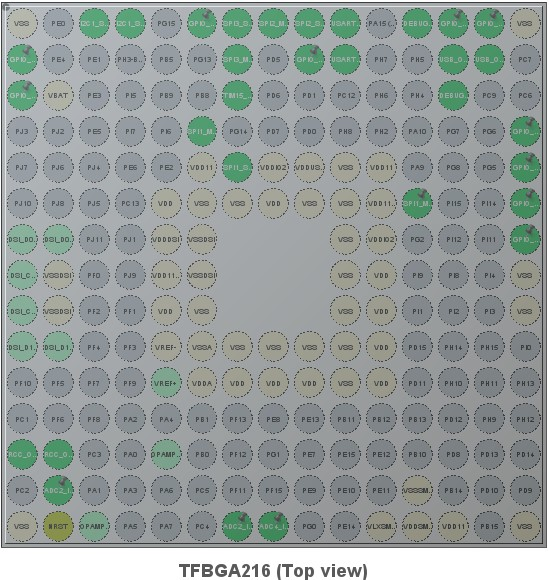
\includegraphics[scale=0.60]{STM32CubeIde.jpg}
			\caption{STM32CubeIDE konfigurace pinů mikrokontroléru} 
			\label{fig:STM32CubeIde}
		\end{subfigure}
		\begin{subfigure}{0.5\textwidth}
				\centering
			\captionsetup{justification=centering}
			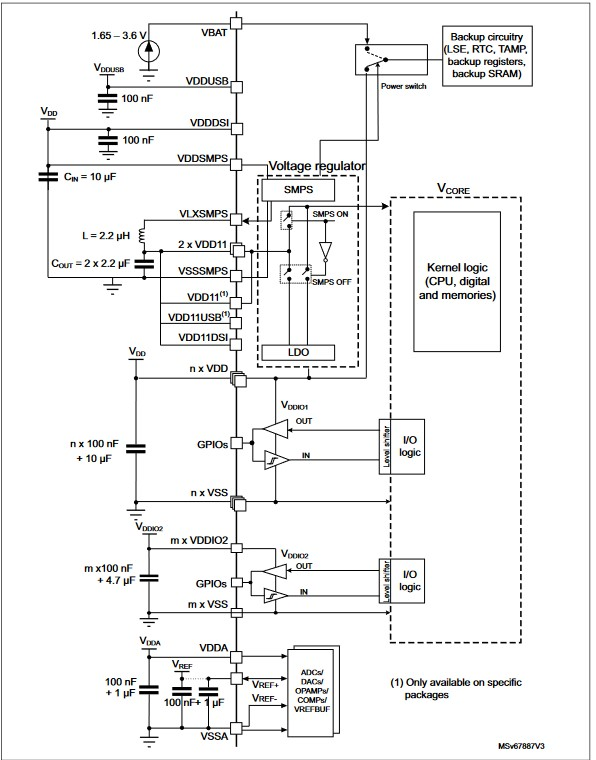
\includegraphics[scale=0.60]{STM32_napajeni.jpg}
			\caption{STM32U5A9 napájení} 
			\label{fig:napajeni_stm32}
		\end{subfigure}
		\caption{Konfigurace a napájení STM32U5A9}
		\label{fig:konfig}
	\end{figure} 
	\begin{table}[h!]
		\centering
		\begin{tabular}{ |P{3cm}||P{10cm}|  }
			\hline
			\multicolumn{2}{|c|}{Napájení základní desky vyčítacího rozhraní} \\
			\hline
			Napájení  & Popis\\ \hline \hline 
			VBAT & Napájení z externí baterie 1.65 - 3.6 V\\ \hline		
			VDDUSB & Napájení periférie USB\\ \hline 		 
			VDDSI & Napájení pro periféri DSI \\ \hline
			VDDSMPS & Napájení pro integrovaný spínaný stabilizátor\\ \hline
			VLXSMPS & Spínaný výstup integrovaného stabilizátoru \\ \hline
			VDD11 & Napájení digitální části mikrokotroléru \\ \hline 
			VDD11, VDD & Napájení digitální části mikrokotroléru ze spínaného stab.\\ \hline
			VDDIO2 & Napájení samostatné vstupní/výstupní brány \\ \hline
			VDDA & Napájení analogové části mikrokotroléru \\ \hline
		\end{tabular}
		\caption{Napájení mikrokontroléru STM32U5A9}
		\label{tab:napajeni_stm32}
	\end{table}
	Výhodou vybraného mikrokontroléru je, že pro napájení jádra a digitálních periferií využívá spínaného regulátoru, který má nižší spotřebu oproti lineárnímu regulátoru, integrovaného přímo na čipu. Nevýhodou je požadavek připojení externí cívky, která je nezbytná pro provoz interního spínaného stabilizátoru. 
	\subsubsection{Hodiny} %Pro USB HS plus konfigurace ostatnich periferii ?
	\subsubsection{PCB}
	Na obrázku \ref{fig:ST_layout} můžete vidět realizaci PCB pro část mikrokontroléru. Nejsou zde uvedeny 2 zbylé vrstvy PCB, kterými jsou 2., 3. a 5. vrstva. Vrstva 2 a 5 tvoří pod částí mikrokontroléru souvislou zemní plochu a vrstva 3 slouží jako vrstva signálová. Blokovací kondenzátory napájení dle specifikací \cite{STM32U5A9_RM} jsou umístěny co nejblíže příslušným pinům, viz. \ref{fig:ST_BOT}. 
	\begin{figure}[h!]
		\centering
		\captionsetup{justification=centering}
		\begin{subfigure}[b]{0.3\textwidth}
			\centering
			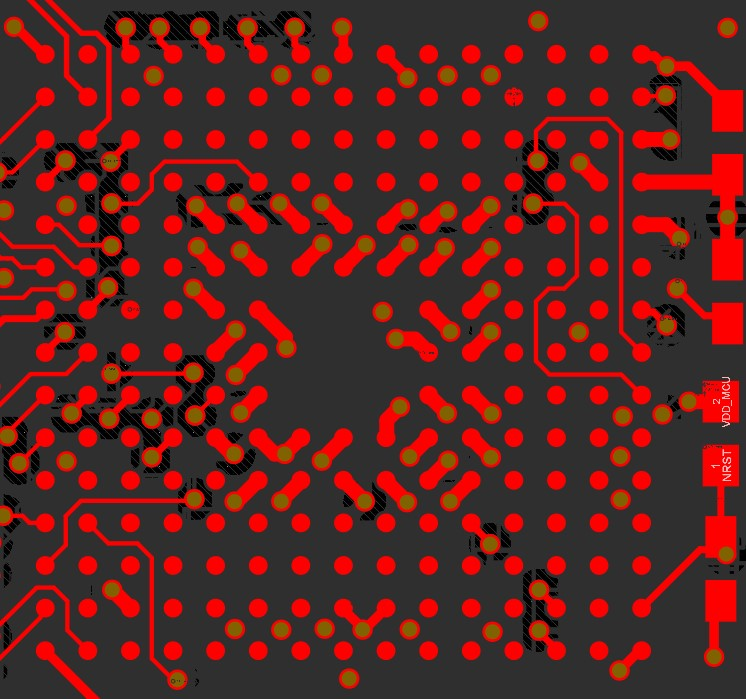
\includegraphics[scale=0.30]{ST_TOP.jpg}
			\caption{Vrchní vrstva PCB STM32U5A9}
			\label{fig:ST_TOP}
		\end{subfigure}
		\hfill
		\begin{subfigure}[b]{0.3\textwidth}
			\centering
				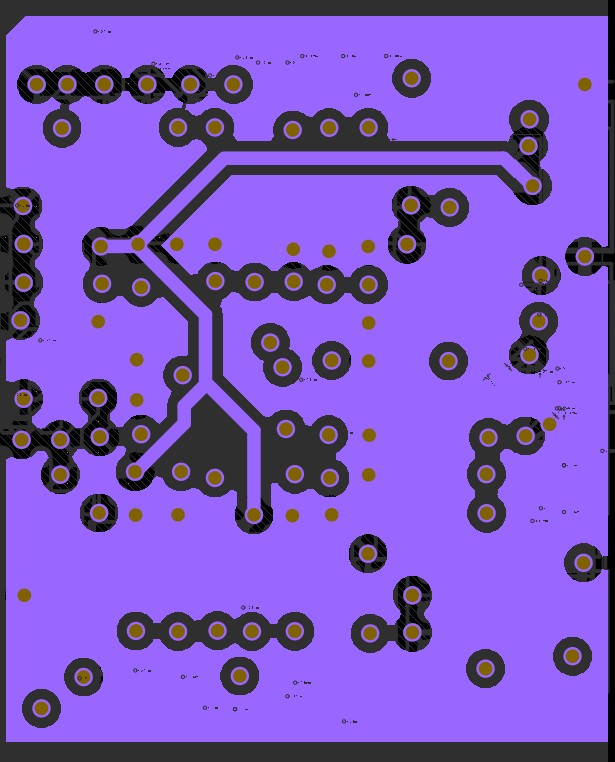
\includegraphics[scale=0.30]{ST_PWR.jpg}
			\caption{Prostřední vrstva PCB STM32U5A9}
			\label{fig:ST_PWR}
		\end{subfigure}
		\hfill
		\begin{subfigure}[b]{0.3\textwidth}
			\centering
				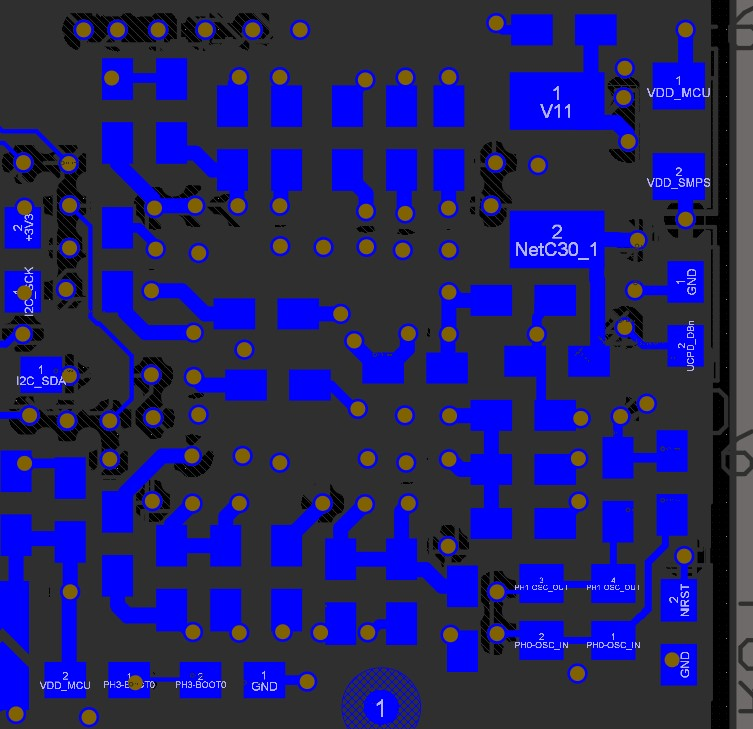
\includegraphics[scale=0.30]{ST_BOT.jpg}
			\caption{Spodní vrstva pcb STM32U5A9}
			\label{fig:ST_BOT}
		\end{subfigure}
		\caption{STM32U5A9 PCB realizace}
		\label{fig:ST_layout}
	\end{figure}
	
	\subsection{Konverze logických úrovní}	% CPLDcko - delice, urovne. Odporove site
	\subsection{USB} % Navrh plosnaku, USB C ochrana, popis USB C konektoru
	\label{USB}

%TODO kde popisu cely cyklus vycitani? v Testovani?
\section{Deska s Timepix 2}
	\subsection{Timepix 2}	% 
		\subsubsection{Rozhraní pro připojení Timepix 2}	% wirebondovaci plosky, HV zdroj
		\subsubsection{Napájení}	% popsat jak se bere z konektoru plus prepinani pro chipID
	\subsection{Vysokonapěťový zdroj}	% MAX1932 zapojeni vysvetleni
		\subsubsection{Měření vysokého napětí} % napetovy sledovac plus konfigurace AD v STM32
	\subsection{Měření teploty}	% proces nastaveni senzoru atd
	\subsection{Konektor}	% popis konektoru, zarazeni zmneni mezi piny
	\label{konektor}
